% Created by tikzDevice version 0.12
% !TEX encoding = UTF-8 Unicode
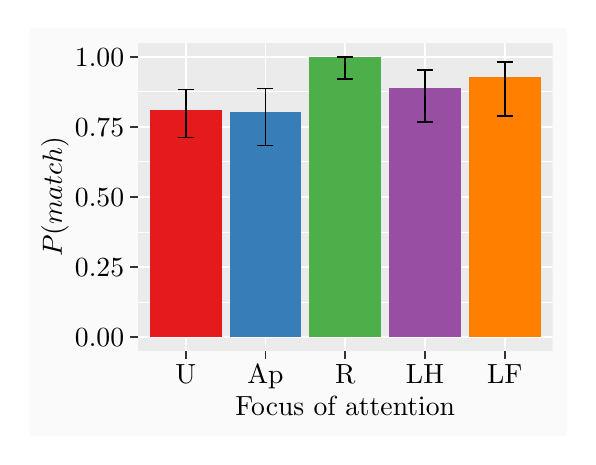
\begin{tikzpicture}[x=1pt,y=1pt]
\definecolor{fillColor}{RGB}{255,255,255}
\path[use as bounding box,fill=fillColor,fill opacity=0.00] (0,0) rectangle (195.19,147.70);
\begin{scope}
\path[clip] (  0.00,  0.00) rectangle (195.19,147.70);
\definecolor{drawColor}{RGB}{255,255,255}
\definecolor{fillColor}{gray}{0.98}

\path[draw=drawColor,line width= 0.6pt,line join=round,line cap=round,fill=fillColor] (  0.00,  0.00) rectangle (195.19,147.70);
\end{scope}
\begin{scope}
\path[clip] ( 39.80, 30.86) rectangle (189.69,142.20);
\definecolor{fillColor}{gray}{0.92}

\path[fill=fillColor] ( 39.80, 30.86) rectangle (189.69,142.20);
\definecolor{drawColor}{RGB}{255,255,255}

\path[draw=drawColor,line width= 0.3pt,line join=round] ( 39.80, 48.58) --
	(189.69, 48.58);

\path[draw=drawColor,line width= 0.3pt,line join=round] ( 39.80, 73.88) --
	(189.69, 73.88);

\path[draw=drawColor,line width= 0.3pt,line join=round] ( 39.80, 99.19) --
	(189.69, 99.19);

\path[draw=drawColor,line width= 0.3pt,line join=round] ( 39.80,124.49) --
	(189.69,124.49);

\path[draw=drawColor,line width= 0.6pt,line join=round] ( 39.80, 35.92) --
	(189.69, 35.92);

\path[draw=drawColor,line width= 0.6pt,line join=round] ( 39.80, 61.23) --
	(189.69, 61.23);

\path[draw=drawColor,line width= 0.6pt,line join=round] ( 39.80, 86.53) --
	(189.69, 86.53);

\path[draw=drawColor,line width= 0.6pt,line join=round] ( 39.80,111.84) --
	(189.69,111.84);

\path[draw=drawColor,line width= 0.6pt,line join=round] ( 39.80,137.14) --
	(189.69,137.14);

\path[draw=drawColor,line width= 0.6pt,line join=round] ( 57.10, 30.86) --
	( 57.10,142.20);

\path[draw=drawColor,line width= 0.6pt,line join=round] ( 85.92, 30.86) --
	( 85.92,142.20);

\path[draw=drawColor,line width= 0.6pt,line join=round] (114.75, 30.86) --
	(114.75,142.20);

\path[draw=drawColor,line width= 0.6pt,line join=round] (143.57, 30.86) --
	(143.57,142.20);

\path[draw=drawColor,line width= 0.6pt,line join=round] (172.39, 30.86) --
	(172.39,142.20);
\definecolor{fillColor}{RGB}{228,26,28}

\path[fill=fillColor] ( 44.13, 35.92) rectangle ( 70.07,118.02);
\definecolor{fillColor}{RGB}{55,126,184}

\path[fill=fillColor] ( 72.95, 35.92) rectangle ( 98.89,117.21);
\definecolor{fillColor}{RGB}{77,175,74}

\path[fill=fillColor] (101.77, 35.92) rectangle (127.72,137.14);
\definecolor{fillColor}{RGB}{152,78,163}

\path[fill=fillColor] (130.60, 35.92) rectangle (156.54,125.90);
\definecolor{fillColor}{RGB}{255,127,0}

\path[fill=fillColor] (159.42, 35.92) rectangle (185.36,129.74);
\definecolor{drawColor}{RGB}{0,0,0}

\path[draw=drawColor,line width= 0.6pt,line join=round] ( 54.22,125.31) --
	( 59.98,125.31);

\path[draw=drawColor,line width= 0.6pt,line join=round] ( 57.10,125.31) --
	( 57.10,107.99);

\path[draw=drawColor,line width= 0.6pt,line join=round] ( 54.22,107.99) --
	( 59.98,107.99);

\path[draw=drawColor,line width= 0.6pt,line join=round] ( 83.04,125.70) --
	( 88.80,125.70);

\path[draw=drawColor,line width= 0.6pt,line join=round] ( 85.92,125.70) --
	( 85.92,105.08);

\path[draw=drawColor,line width= 0.6pt,line join=round] ( 83.04,105.08) --
	( 88.80,105.08);

\path[draw=drawColor,line width= 0.6pt,line join=round] (111.86,137.14) --
	(117.63,137.14);

\path[draw=drawColor,line width= 0.6pt,line join=round] (114.75,137.14) --
	(114.75,129.05);

\path[draw=drawColor,line width= 0.6pt,line join=round] (111.86,129.05) --
	(117.63,129.05);

\path[draw=drawColor,line width= 0.6pt,line join=round] (140.69,132.49) --
	(146.45,132.49);

\path[draw=drawColor,line width= 0.6pt,line join=round] (143.57,132.49) --
	(143.57,113.54);

\path[draw=drawColor,line width= 0.6pt,line join=round] (140.69,113.54) --
	(146.45,113.54);

\path[draw=drawColor,line width= 0.6pt,line join=round] (169.51,135.21) --
	(175.27,135.21);

\path[draw=drawColor,line width= 0.6pt,line join=round] (172.39,135.21) --
	(172.39,115.88);

\path[draw=drawColor,line width= 0.6pt,line join=round] (169.51,115.88) --
	(175.27,115.88);
\end{scope}
\begin{scope}
\path[clip] (  0.00,  0.00) rectangle (195.19,147.70);
\definecolor{drawColor}{RGB}{0,0,0}

\node[text=drawColor,anchor=base east,inner sep=0pt, outer sep=0pt, scale=  1.00] at ( 34.85, 32.48) {0.00};

\node[text=drawColor,anchor=base east,inner sep=0pt, outer sep=0pt, scale=  1.00] at ( 34.85, 57.78) {0.25};

\node[text=drawColor,anchor=base east,inner sep=0pt, outer sep=0pt, scale=  1.00] at ( 34.85, 83.09) {0.50};

\node[text=drawColor,anchor=base east,inner sep=0pt, outer sep=0pt, scale=  1.00] at ( 34.85,108.39) {0.75};

\node[text=drawColor,anchor=base east,inner sep=0pt, outer sep=0pt, scale=  1.00] at ( 34.85,133.70) {1.00};
\end{scope}
\begin{scope}
\path[clip] (  0.00,  0.00) rectangle (195.19,147.70);
\definecolor{drawColor}{gray}{0.20}

\path[draw=drawColor,line width= 0.6pt,line join=round] ( 37.05, 35.92) --
	( 39.80, 35.92);

\path[draw=drawColor,line width= 0.6pt,line join=round] ( 37.05, 61.23) --
	( 39.80, 61.23);

\path[draw=drawColor,line width= 0.6pt,line join=round] ( 37.05, 86.53) --
	( 39.80, 86.53);

\path[draw=drawColor,line width= 0.6pt,line join=round] ( 37.05,111.84) --
	( 39.80,111.84);

\path[draw=drawColor,line width= 0.6pt,line join=round] ( 37.05,137.14) --
	( 39.80,137.14);
\end{scope}
\begin{scope}
\path[clip] (  0.00,  0.00) rectangle (195.19,147.70);
\definecolor{drawColor}{gray}{0.20}

\path[draw=drawColor,line width= 0.6pt,line join=round] ( 57.10, 28.11) --
	( 57.10, 30.86);

\path[draw=drawColor,line width= 0.6pt,line join=round] ( 85.92, 28.11) --
	( 85.92, 30.86);

\path[draw=drawColor,line width= 0.6pt,line join=round] (114.75, 28.11) --
	(114.75, 30.86);

\path[draw=drawColor,line width= 0.6pt,line join=round] (143.57, 28.11) --
	(143.57, 30.86);

\path[draw=drawColor,line width= 0.6pt,line join=round] (172.39, 28.11) --
	(172.39, 30.86);
\end{scope}
\begin{scope}
\path[clip] (  0.00,  0.00) rectangle (195.19,147.70);
\definecolor{drawColor}{RGB}{0,0,0}

\node[text=drawColor,anchor=base,inner sep=0pt, outer sep=0pt, scale=  1.00] at ( 57.10, 19.03) {U};

\node[text=drawColor,anchor=base,inner sep=0pt, outer sep=0pt, scale=  1.00] at ( 85.92, 19.03) {Ap};

\node[text=drawColor,anchor=base,inner sep=0pt, outer sep=0pt, scale=  1.00] at (114.75, 19.03) {R};

\node[text=drawColor,anchor=base,inner sep=0pt, outer sep=0pt, scale=  1.00] at (143.57, 19.03) {LH};

\node[text=drawColor,anchor=base,inner sep=0pt, outer sep=0pt, scale=  1.00] at (172.39, 19.03) {LF};
\end{scope}
\begin{scope}
\path[clip] (  0.00,  0.00) rectangle (195.19,147.70);
\definecolor{drawColor}{RGB}{0,0,0}

\node[text=drawColor,anchor=base,inner sep=0pt, outer sep=0pt, scale=  1.00] at (114.75,  7.44) {Focus of attention};
\end{scope}
\begin{scope}
\path[clip] (  0.00,  0.00) rectangle (195.19,147.70);
\definecolor{drawColor}{RGB}{0,0,0}

\node[text=drawColor,rotate= 90.00,anchor=base,inner sep=0pt, outer sep=0pt, scale=  1.00] at ( 12.39, 86.53) {\(P(match)\)};
\end{scope}
\end{tikzpicture}
